\subsection{\textit{Dropout} tikimybės įtaka}
\label{subsec:rez_dropout}

Tikrinamos keturios \textit{Dropout} tikimybės: $0$, $0{,}25$, $0{,}5$ ir $0{,}75$. Architektūra pagal nutylėjimą (vaizdams \texttt{(32, 64, 128)}, laiko eilutėms \texttt{(64, 128)}). Rezultatai pateikti~\ref{tab:rez_dropout} lentelėje, validavimo metrikos – \ref{fig:rez_dropout_image} ir~\ref{fig:rez_dropout_keystroke} pav.

\begin{table}[H]
    \centering
    \caption{\textit{Dropout} tikimybės tyrimo rezultatai. Geriausi variantai paryškinti.}
    \begin{tabular}{|l|l|c|c|c|}
        \hline
        Užduotis & Tikimybė & \texttt{val\_acc} & \texttt{val\_loss} & \texttt{test\_acc} \\
        \hline
        \multirow{4}{*}{Vaizdai}
            & \textbf{$0{,}00$} & $\mathbf{0{,}8466}$ & $0{,}8865$ & $\mathbf{0{,}8347}$ \\ \cline{2-5}
            & $0{,}25$ & $0{,}8095$ & $0{,}4478$ & $0{,}8093$ \\ \cline{2-5}
            & $0{,}50$ & $0{,}7989$ & $\mathbf{0{,}4459}$ & $0{,}7924$ \\ \cline{2-5}
            & $0{,}75$ & $0{,}6667$ & $0{,}6780$ & $0{,}5763$ \\
        \hline
        \multirow{4}{*}{Laiko eilutės}
            & \textbf{$0{,}00$} & $\mathbf{0{,}7125}$ & $\mathbf{0{,}9609}$ & $\mathbf{0{,}7533}$ \\ \cline{2-5}
            & $0{,}25$ & $0{,}6750$ & $1{,}1523$ & $0{,}7167$ \\ \cline{2-5}
            & $0{,}50$ & $0{,}6000$ & $1{,}6406$ & $0{,}6767$ \\ \cline{2-5}
            & $0{,}75$ & $0{,}0917$ & $3{,}3900$ & $0{,}0600$ \\
        \hline
    \end{tabular}
    \label{tab:rez_dropout}
\end{table}


\begin{figure}[H]
    \centering
    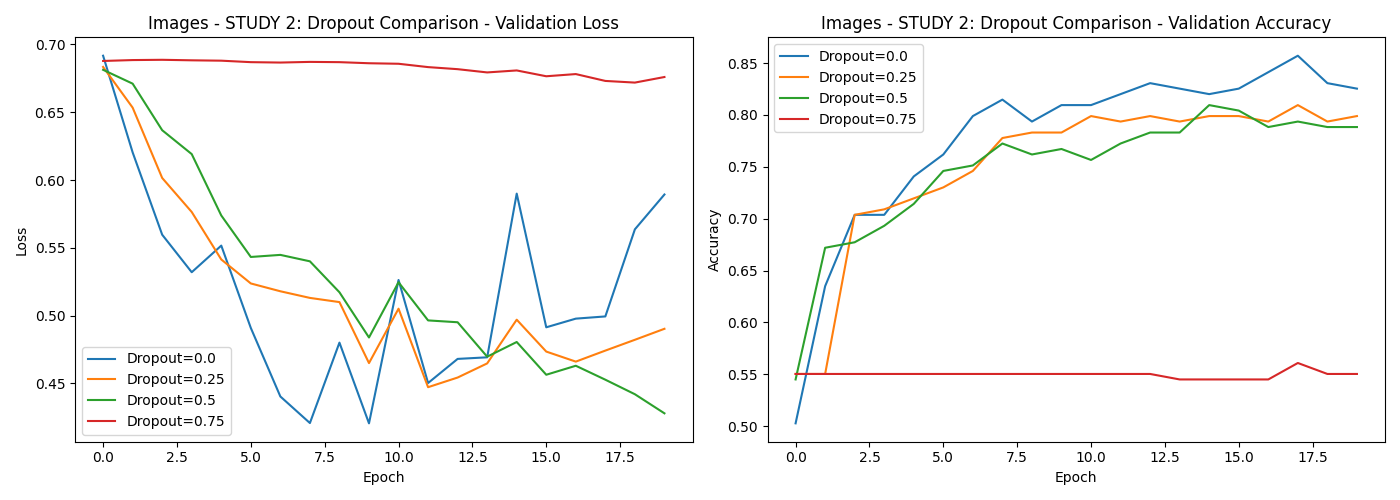
\includegraphics[width=0.9\linewidth]{3Lab/results/dropout/img_comparison.png}
    \caption{\textit{Dropout} tyrimas – vaizdų užduotis}
    \label{fig:rez_dropout_image}
\end{figure}

\begin{figure}[H]
    \centering
    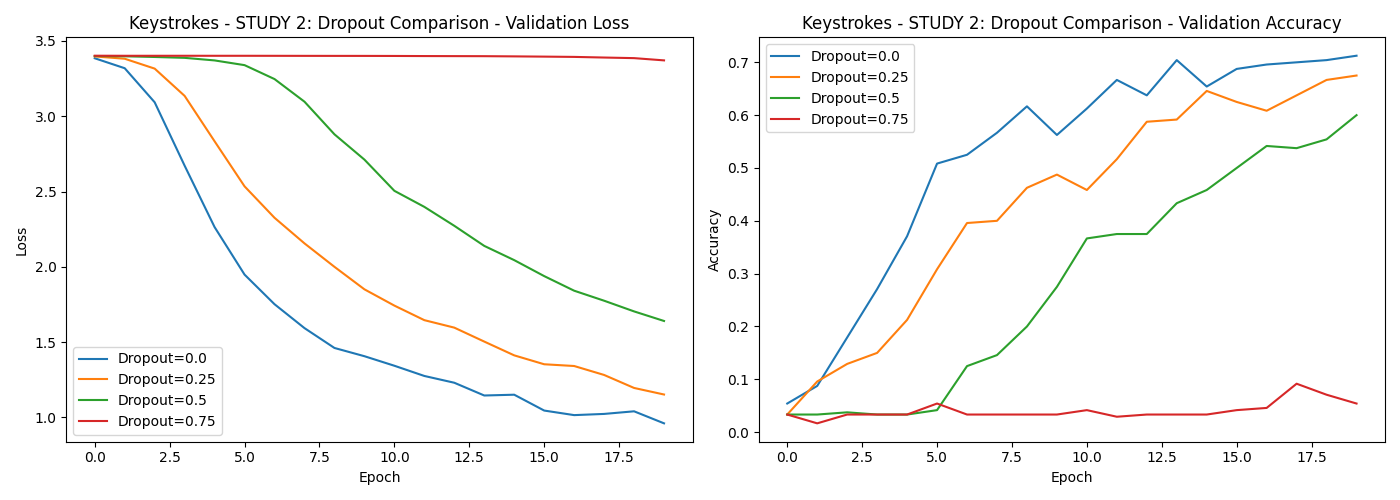
\includegraphics[width=0.9\linewidth]{3Lab/results/dropout/ks_comparison.png}
    \caption{\textit{Dropout} tyrimas – laiko eilučių užduotis}
    \label{fig:rez_dropout_keystroke}
\end{figure}

Pastebimi rezultatai:
\begin{itemize}
    \item Abiem užduotims \textbf{tikimybė $0{,}0$} davė geriausią validavimo tikslumą, nes mokymo aibės yra nedidelės ir tinklas nepasiekia stipraus persimokymo. Padidinus tikimybę iki $0{,}5$ tikslumas krenta, bet ne katastrofiškai.
    \item \textbf{Tikimybė $0{,}75$} sunaikina mokymo signalą – laiko eilučių modelis nepasiekia net $10\,\%$ tikslumo (kas yra atsitiktinio spėjimo lygis $30$ klasių užduotyje).
    \item Vaizdams su \texttt{Dropout}~$=0{,}5$ \texttt{val\_loss} ($0{,}4459$) yra mažiausias, todėl jei svarbi prognozės pasitikėjimo kalibracija, ši tikimybė geriausia – tačiau kelia mažesnį tikslumą.
\end{itemize}
